\documentclass[]{article}
\usepackage{amsmath}
\usepackage{amsthm}
\usepackage{amssymb}
\usepackage{graphicx}
\usepackage{float}
\usepackage{listings}
\usepackage{caption}
\usepackage{subcaption}
\usepackage[round]{natbib}
\bibliographystyle{unsrtnat}

%\usepackage{multicol}
%\usepackage{bm}
%\usepackage{physics}

% this just sets up the page size and margins
\setlength{\topmargin}{0pt}
\setlength{\oddsidemargin}{0pt}
\setlength{\evensidemargin}{0pt}
\setlength{\textwidth}{6.5in}
\setlength{\textheight}{8.5in}
\setlength{\headheight}{0pt}

%%%%%%%%%%%%%%%%%%%%%%%%%%%%%%%%%%%%%%%%%%%%%%%%
%
%  This is all the stuff for Python code snippets
%
\DeclareFixedFont{\ttb}{T1}{txtt}{bx}{n}{10} % for bold
\DeclareFixedFont{\ttm}{T1}{txtt}{m}{n}{10}  % for normal
% Custom colors
\usepackage{color}
\definecolor{deepblue}{rgb}{0,0,0.5}
\definecolor{deepred}{rgb}{0.6,0,0}
\definecolor{deepgreen}{rgb}{0,0.5,0}

\setcounter{MaxMatrixCols}{15}

% Python style for highlighting
\newcommand\pythonstyle{\lstset{
		language=Python,
		basicstyle=\ttm,
		morekeywords={self},              % Add keywords here
		keywordstyle=\ttb\color{deepblue},
		emph={MyClass,__init__},          % Custom highlighting
		emphstyle=\ttb\color{deepred},    % Custom highlighting style
		stringstyle=\color{deepgreen},
		frame=tb,                         % Any extra options here
		showstringspaces=false,
		tabsize=4
}}

% Python environment
\lstnewenvironment{python}[1][]
{
	\pythonstyle
	\lstset{#1}
}
{}

% Python for inline
\newcommand\pythoninline[1]{{\pythonstyle\lstinline!#1!}}

%%%%%%%%%%%%%%%%%%%%%%%%%%%%%%%%%%%%%%%%%%%%%%%%%


\newcommand{\mpc}{MPC}
\newcommand{\nmpc}{NMPC}
\newcommand{\pdiff}{P_{\Delta}}
\newcommand{\pavg}{\overline{P}}
\newcommand{\R}{\mathbb{R}}
\newcommand{\casadi}{CasADi}
\newcommand{\dompc}{{\bf do-mpc}}

\title{NMPC Applied to a Thrust-Vector-Controlled Drone}
\author{Isidore Mones and Heidi Dixon}
%\date{}

\begin{document}
\maketitle

\section*{Introduction}

\section*{Hardware and Design}

The thrust-vectoring drone was designed as a low-cost, modular research platform for testing nonlinear model predictive control algorithms on a physical flight system. The vehicle design is inspired by the EPFL thrust-vectoring research drone \cite{TVCDrone}, with an emphasis on repairability, ease of modification, and compatibility with common off-the-shelf flight hardware.
Our drone has a total mass of 1.5 kg, and a diameter and height of 260mm and 500 mm respectively.
The propellers are collinear and counter-rotating to allow for yaw controllability. They are driven by BrotherHobby 2207 BLDC motor. The vehicle center of mass is located near the central body axis, with its exact position determined primarily by the placement of the battery, onboard computer, flight controller, and power electronics. The thrust vector angles are are actuated using a two axis gimbal with PDI-6621MG servos.

Onboard computation is split between a Raspberry Pi 5 and a Pixhawk 4 flight controller. The Raspberry Pi 5 runs the nonlinear model predictive controller, while the Pixhawk 4 handles sensor fusion and actuator command passthrough. State estimation is performed using the Pixhawk’s onboard Extended Kalman Filter, which fuses measurements from the onboard IMU, barometer, magnetometer, GPS, and optical-flow sensor.

The electrical system uses a 6S battery to power the propulsion system through approximately 45 A Tekko32 ESCs driving the BLDC motors. Power and PWM distribution are handled by a PM-07 power and PWM distribution board. A Pololu 5 V buck converter supplies regulated power to the Raspberry Pi and servo electronics. This power architecture separates high-current motor power from the lower-voltage computation and actuation electronics, improving reliability and simplifying troubleshooting.

For navigation, the drone uses the Pixhawk onboard IMU, barometer, and magnetometer, along with an M9N GPS for outdoor positioning and an ARK Flow MR optical-flow sensor for indoor or GPS-denied flight. The ARK Flow MR is a DroneCAN optical-flow, distance-sensor, and IMU module designed for mid-range applications, allowing the Pixhawk EKF to improve state estimation when GPS measurements are unavailable or unreliable.

Communication between the controller on the Raspberry Pi and the Pixhawk is handled through ROS 2 running on Ubuntu 24.04 LTS. The Raspberry Pi sends actuator commands to the Pixhawk, allowing the NMPC controller to command the propulsion and thrust-vectoring system through the Pixhawk interface. This architecture allows the computationally expensive control algorithm to run on the Raspberry Pi while preserving the Pixhawk’s robust sensor fusion and hardware interfacing capabilities.

Overall, the hardware platform was designed to balance research capability with practical constraints. The use of 3D-printed gimbals, commercially available flight electronics, and a modular power architecture makes the vehicle inexpensive to repair while still providing sufficient onboard computation and sensing for advanced control experiments.

\section*{Model}


\section*{PixHawk Configuration}

\section*{Reference Frames}


\section*{Thrust Testing}

\begin{figure}[H]
	\centering
	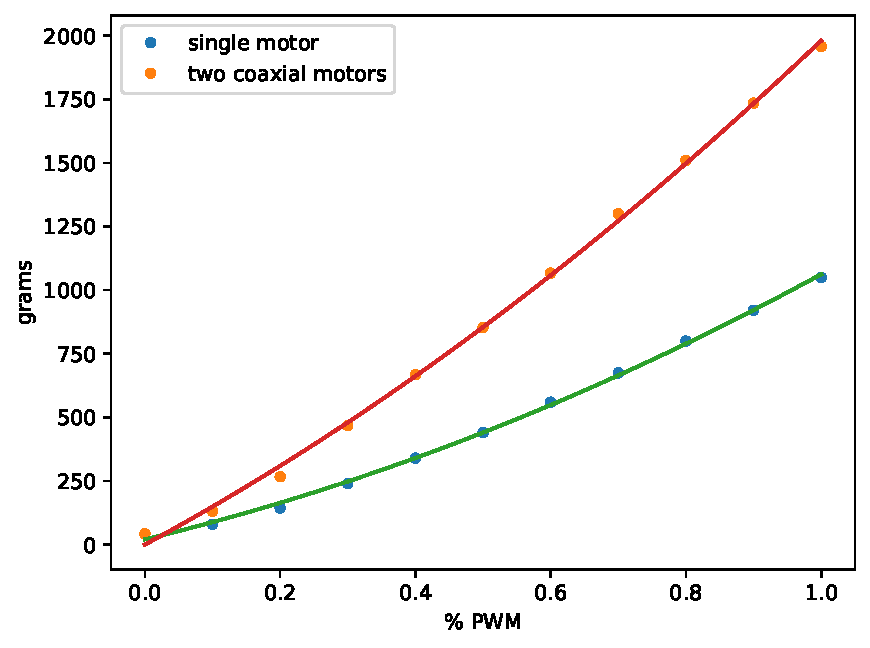
\includegraphics[width=\textwidth]{figures/thrust_test_graph.pdf}
	\caption{Pulse width modulation value from $0-1$ versus thrust measured in grams for a single motor and two coaxial motors. Each thrust profile is fitted with a quadratic curve.}
	\label{fig:thrust_test}
\end{figure}

\section*{Algorithms}
\subsection*{Software Architecture}

\subsection*{NMPC}
\subsection*{NPL Formulation}

\section*{Experimental Results}
\section*{Conclusions}

	


\bibliography{references.bib}
\end{document}

